  \documentclass{journal}[IEEEtran, twocolumn]             % No modificar

% PASO 1. Reemplace "Práctica 1" por el número de la práctica que corresponda
\newcommand{\dochead}{Practice N°3}     

% PASO 2. Verifique el título de la práctica corresponda.
\newcommand{\docsubhead}{RF-EC Conversion}  

% PASO 3. Reemplace "B1A - 02" por el grupo de la asignatura y el número de su grupo de laboratorio
\newcommand{\teamname}{A1}     

% PASO 4. OPCIONAL: Reemplace "\docsubhead \docsubhead" por el título del documento en caso de requerirse.
\newcommand{\titulo}{\dochead: \docsubhead}      

% PASO 5. Reemplace "31 de diciembre de 2030" por la fecha de su documento
\newcommand{\fecha}{October 5, 2025}      

% To load packages
\usepackage{microtype}
\usepackage[T1]{fontenc}
\usepackage[utf8]{inputenc} 
\usepackage[english]{babel}
\usepackage[letterpaper,left=2.0cm,top=2.0cm,right=2.0cm,bottom=4.0cm]{geometry}
\usepackage{amsmath}
\usepackage{amsfonts}
\usepackage{fancyhdr}
\usepackage{fancyvrb}
\usepackage{listings}
\usepackage{array}
\usepackage{graphicx,color,enumerate}	
\usepackage{multirow} 
\usepackage{multicol}
\usepackage{authblk}
\usepackage{charter}    
\usepackage{titling}
\usepackage{url}
\usepackage{hyperref}
\usepackage{xcolor}
\usepackage{tabularx}
\usepackage{tikz}
\usepackage{float}
\usepackage{booktabs}
\usepackage{longtable}
\usepackage{adjustbox}
\usepackage{subcaption}
\usepackage{colortbl}
\usepackage{tcolorbox}
\usepackage{enumitem}

\definecolor{uisgreen}{RGB}{125,194,3}
\definecolor{gray97}{gray}{.97}
\definecolor{gray75}{gray}{.75}
\definecolor{gray45}{gray}{.45}

\setlength{\droptitle}{-1.8cm}
\pagestyle{fancy}

%%% Header definition
\headheight=60pt 						% header height 
\renewcommand{\headrulewidth}{4pt}
\let\oldheadrule\headrule% Copy \headrule into \oldheadrule
\renewcommand{\headrule}{\color{uisgreen}\oldheadrule}

\fancyhead[L]							% left header 
{	\begin{minipage}{2.5cm}
		
\includegraphics[scale=0.3]{./figs/uislogohoriz.png} 
	\end{minipage}	
	\begin{minipage}{5cm}
	    \color{uisgreen}
	    \footnotesize {\textsf{Universidad Industrial de Santander\\ 
				Escuela de Ingenierías Eléctrica, \\
				Electrónica y de Telecomunicaciones	}}	
	\end{minipage}
}
\fancyhead[R] { 							%la "C" indica al centro
	\begin{minipage}{8cm}
	    \color{uisgreen}
	    \begin{flushright}
    	    \small{\textsf{Communications II - LAB (27145)}} \\
            \normalsize{\textsf{\dochead: \textbf{\docsubhead}}} \\
    	    \small{\textsf{Group: \textbf{\teamname}}}
	    \end{flushright}
    \end{minipage}
    \begin{minipage}{1.2cm}
		
\includegraphics[width=1.0\textwidth]{./figs/logoE3T.png} 
	\end{minipage}	
}
%%% End header definition

\lstset{ frame=Ltb,
     framerule=0pt,
     aboveskip=5pt,
     framextopmargin=3pt,
     framexbottommargin=3pt,
     framexleftmargin=0.4cm,
     framesep=0pt,
     rulesep=.4pt,
     backgroundcolor=\color{gray97},
     rulesepcolor=\color{black},
     %
     stringstyle=\ttfamily\color{red!50!brown},
     showstringspaces = false,
     basicstyle=\small\ttfamily,
     commentstyle=\color{gray45},
     keywordstyle=\color{blue}\bfseries,
     %
     numbers=left,
     numbersep=5pt,
     numberstyle=\tiny,
     numberfirstline = false,
     breaklines=true,
   }

% minimizar fragmentado de listados
\lstnewenvironment{listing}[1][]
   {\lstset{#1}\pagebreak[0]}{\pagebreak[0]}

\lstdefinestyle{consola}
   {basicstyle=\scriptsize\bf\ttfamily,
    backgroundcolor=\color{gray75},
   }

\lstdefinestyle{C}
   {language=C,
   }

             % No modificar


\begin{document}                    % No modificar

\title{\textbf{\titulo}}            % No modificar

% PASO 6. Agregar aquí el nombre y código de los autores.  
\author{
Leonel Ricardo Araque - 2204224 \\
Leandro José Garzón - 2194232 \\
\href{https://github.com/leo09p/COMMII_A1_G8/tree/Practica_3}{https://github.com/leo09p/COMMII_A1_G8/tree/Practica_3}
}

\affil{\small{Escuela de Ingenierías Eléctrica, Electrónica y de Telecomunicaciones} \\ % No modificar
\small{Universidad Industrial de Santander}} % No modificar

\date{\fecha}                       % No modificar

\maketitle                          % No modificar
\thispagestyle{fancy}               % No modificar

%---------------------------------------------------------------
% PASO 7. **..**...****INICIE SU DOCUMENTO DESDE AQUI***...**...
%%%%% A PARTIR DE AQUÍ EDITE EL DOCUMENTO PARA AGREGAR TODO EL CONTENIDO REQUERIDO PARA EL ENTREGABLE CORRESPONDIENTE
%%%%  Todo el contenido a partir de este punto es SOLAMENTE ILUSTRATIVO.

\color{black}

\begin{multicols}{2}

\begin{abstract}

This lab analyzes OOK, BPSK, and FSK modulation, both in their RF and complex envelope representations. The block flow is implemented in GNU Radio, and the corresponding diagrams are included in the GitHub repository.

\end{abstract}

\section{Introduction}

The practice is based on RF-EC conversion, with the following objectives:

\begin{enumerate}
    \item Analysis and development of OOK modulation\item Analysis and development of BPSK modulation \item Analysis and development of FSK modulation\item Adressing Control questions
\end{enumerate}

With this on mind, the practice was developed in intervals between various laboratory sessions, where simulations and discussions of their respective behaviors were conducted.

The GNU-Radio tool was used for the development of these components, and a new branch was created on Github to distinguish this practice.

\section{Methodology}

Figure \ref{fig:figA} represents the flowchart designed for the implementation of various proposed modulations. 

\begin{figure}[H]
    \centering
        \centering
        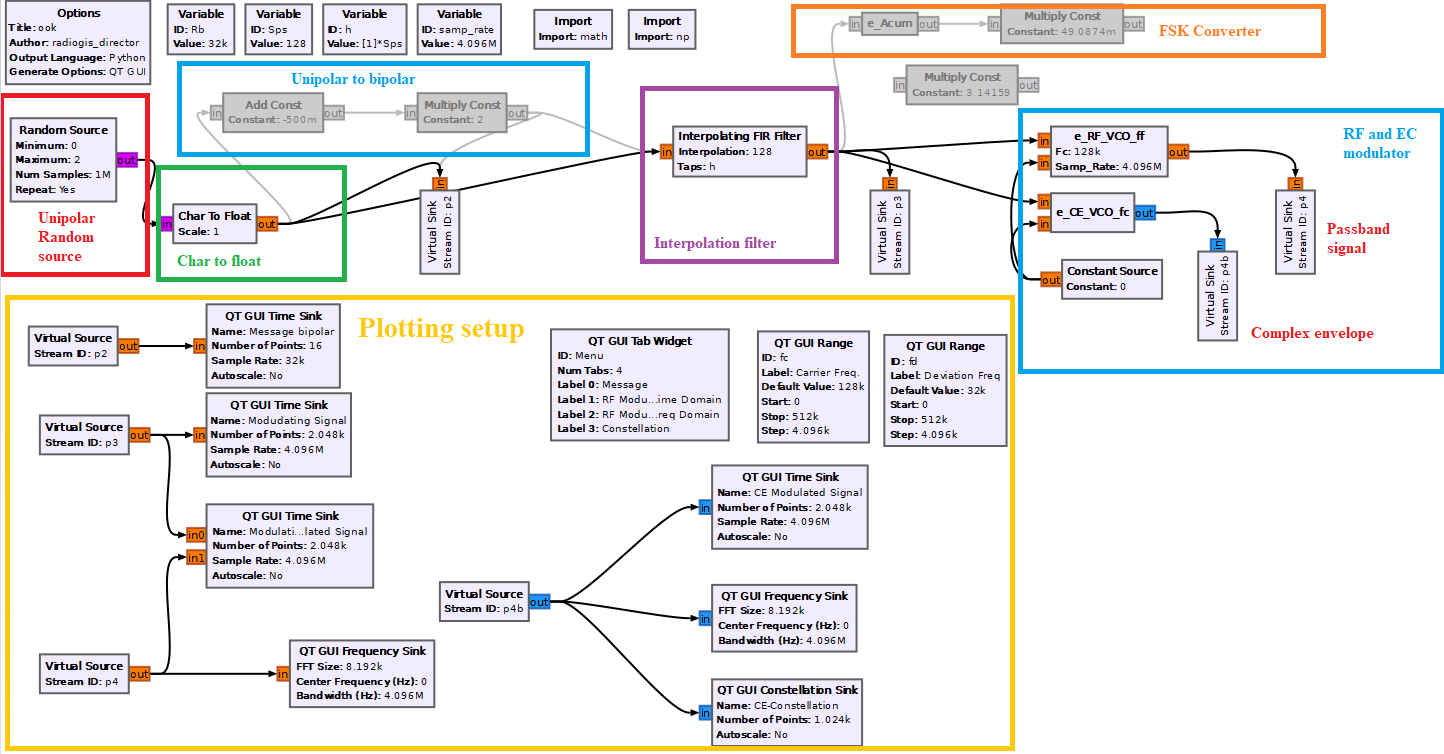
\includegraphics[width=0.6\columnwidth]{figs/Structure.png}
    \caption{System's Flowchart}
    \label{fig:figA}
\end{figure}

Specifically, in the figure, it can be seen the labeling of each respective set of blocks where, based on their meaning, the respective changes were made to achieve one modulation or another. Below, it was described how each modulation was obtained:

\begin{itemize}

\item \textbf{OOK}:
For OOK modulation, the block system was left as originally configured, and the program was run accordingly.

\item \textbf{BPSK}:
For BPSK modulation, the respective offset change of the circuit was performed. For this, the high-value was halved and then multiplied by a factor of 2. In Figure \ref{fig:figA}, it can be seen the marked set of boxes that need to be enabled for this adjustment.

\item \textbf{FSK}:
For FSK modulation, the accumulator block and a multiplicative constant corresponding to the frequency sensitivity coefficient were activated. These are shown in Figure \ref{fig:figA}. With this in mind, now the corresponding analysis could be carried out.

\end{itemize}

Other modifications of figure \ref{fig:figA} which were part of specific objectives were considered, such as modifying the phase to observe its behavior. With all these modifications already made, from the graphing blocks found in the lower area of the flowcharts, the time, frequency, and complex plane components of the signal are plotted. In this case, the first two contain the signal as RF and as EC.

\section{Results and analysis}

The analysis of results was divided as agreed upon in the introduction of the report.

\subsection{OOK}

The analysis of OOK modulation is carried out using two carrier frequencies: 
128 kHz and 256 kHz. In the frequency domain, the change in $f_c$ is reflected in the 
shift of the main lobes generated by the RF-VCO, without being affected by frequency 
deviations, unlike other modulations such as FSK or BPSK. In the time domain, it is 
observed that the carrier is present only when the bit is “1”, while it disappears 
for the bit “0”.

In the complex envelope representation, with a constant phase of $0^\circ$, the message 
appears as completely real, which is evident in the constellation diagram where the 
quadrature component remains equal to zero. This confirms that OOK is a type of 
amplitude modulation in which the information depends exclusively on the presence 
or absence of the carrier, as illustrated in Figure



\ref{fig:figOOK}.

\begin{figure}[H]
    \centering
        \centering
        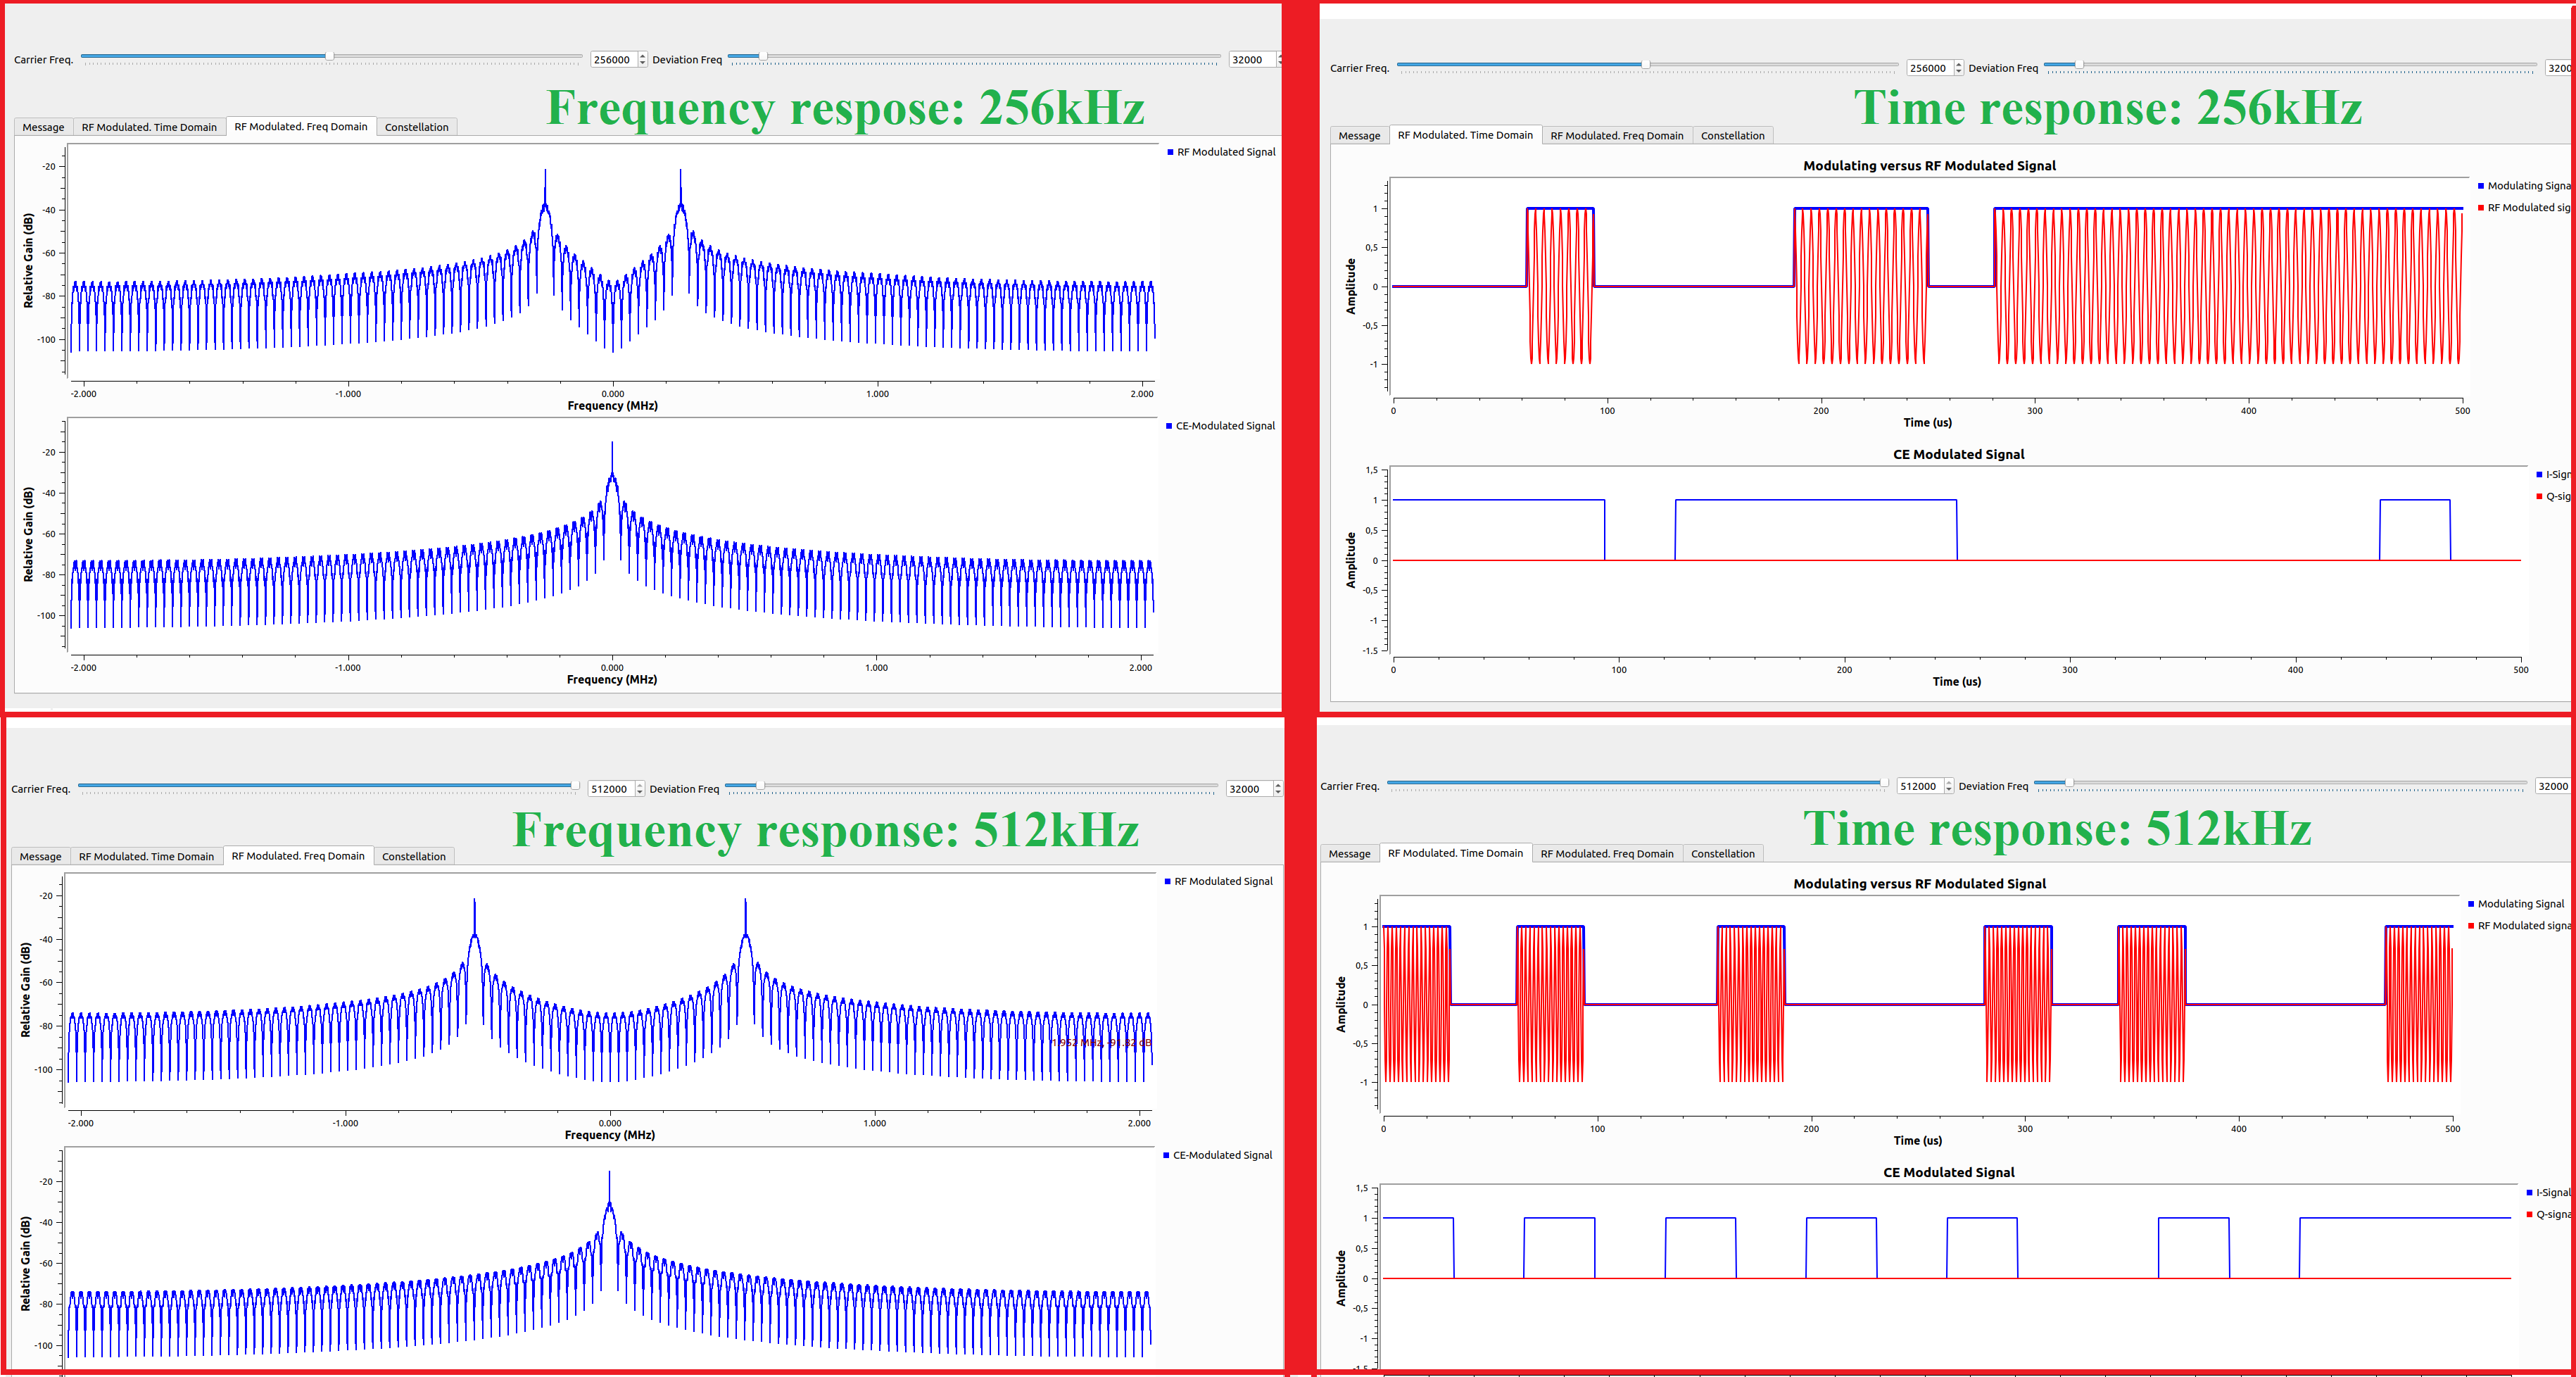
\includegraphics[width=0.7\columnwidth]{figs/OOK.png}
    \caption{OOK modulation}
    \label{fig:figOOK}
\end{figure}
Due to this characteristic, OOK requires less power compared to BPSK and FSK; 
however, it is more sensitive to noise since the information is transmitted only 
through amplitude variations.

\subsection{BPSK}
In BPSK modulation, the transmitted bit determines the phase of the carrier, 
which alternates between $0^\circ$ and $180^\circ$. For the analysis, two carrier 
frequencies are used: 32 kHz and 128 kHz, while keeping the frequency deviation constant. 
The phase is varied between 0 and 1 in order to evaluate its effect on both RF and EC 
representations.

In the RF case, the signal inverts its polarity depending on the transmitted bit, 
producing two states separated by $180^\circ$. In the EC representation, it is observed 
that when the phase is $0^\circ$, the quadrature component $Q$ is equal to zero, since 
the signal remains purely real. When the phase is shifted, the $Q$ component takes 
non-zero values, representing the bipolar nature of the modulation. These behaviors 
are illustrated in Figure\ref{fig:figBPSK}  


\begin{figure}[H]
    \centering
        \centering
        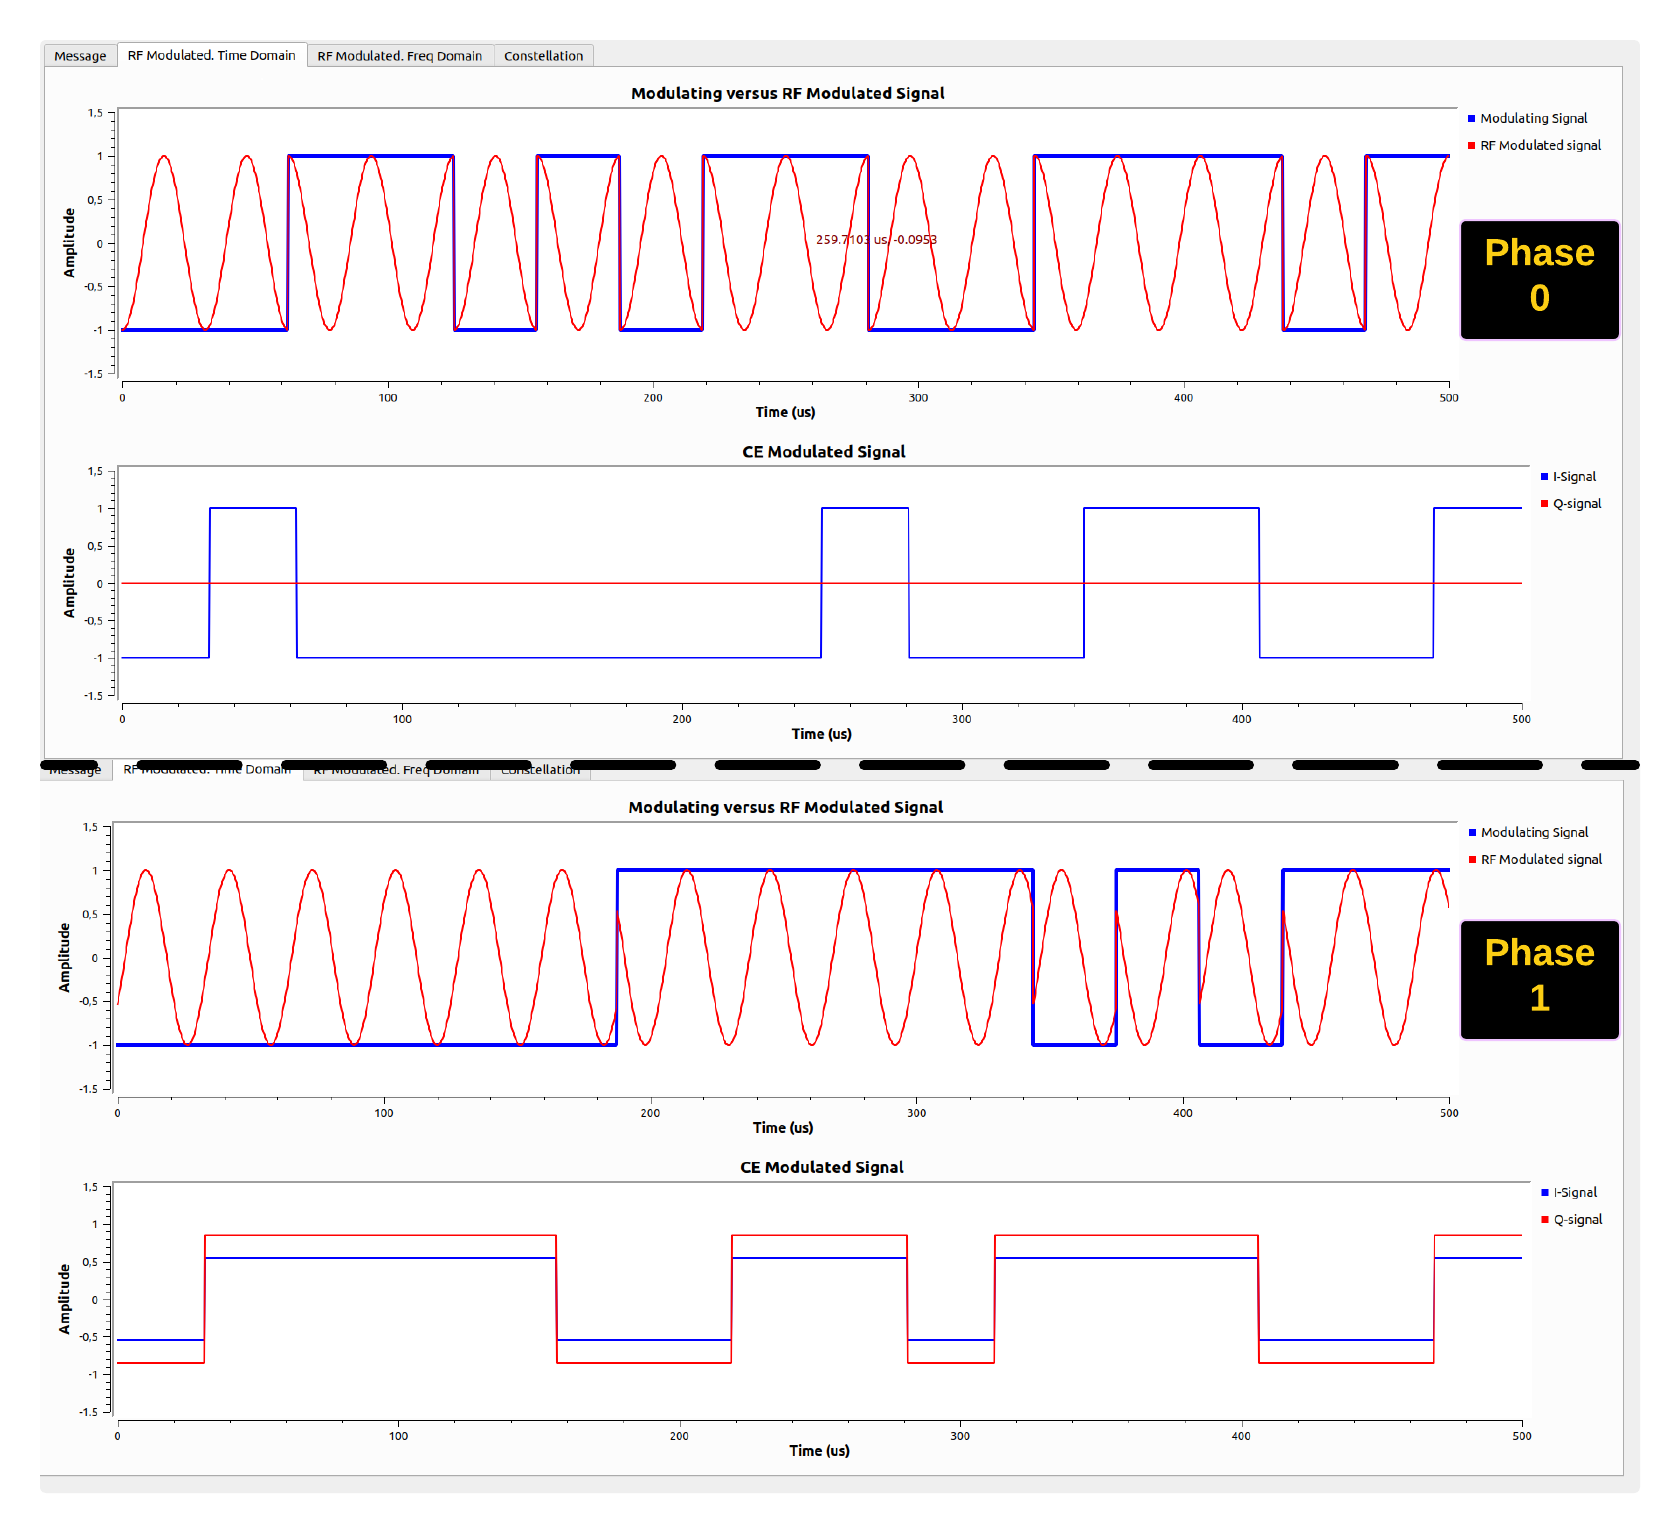
\includegraphics[width=0.6\columnwidth]{figs/BPSK.png}
    \caption{BPSK Modulation}
    \label{fig:figBPSK}
\end{figure}
As a result, BPSK shows greater robustness to noise than OOK, but requires 
synchronization of the carrier phase to correctly distinguish between the two 
possible symbol states.


\subsection{FSK}
For the FSK modulation, the system includes two key modifications: the addition 
of an \texttt{e\_Acum} block, which integrates the input signal, and a 
\texttt{Multiply Constant} block that determines the frequency deviation. 
The modulated signal is applied to the phase input of the VCO, keeping the 
amplitude constant in order to vary the instantaneous frequency according 
to the input bit.

When the carrier frequency ($f_c$) and the frequency deviation ($f_d$) are adjusted, 
different behaviors can be observed. If both values are equal, one of the two 
sinusoidal components becomes constant (zero frequency). On the other hand, 
if $f_c \gg f_d$, the two frequency levels become almost indistinguishable. 
These effects can be seen in Figure~\ref{fig:fsk}, which shows the modulation 
for $f_c = 64$~kHz and $f_d = 80$~kHz.

\begin{figure}[H]
    \centering
        \centering
        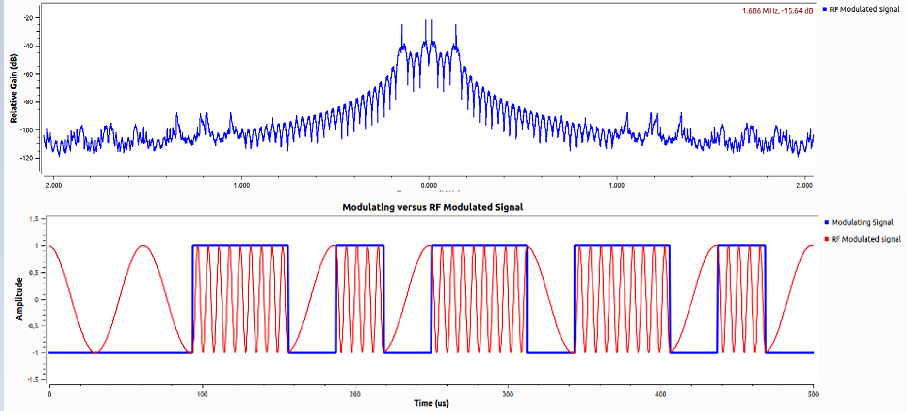
\includegraphics[width=0.6\columnwidth]{figs/FSK.png}
    \caption{FSK Modulation}
    \label{fig:figFSK}
\end{figure}
In the frequency domain, $f_c$ shifts the entire spectrum, while $f_d$ controls 
the separation between the two dominant lobes. A larger frequency deviation 
produces greater separation between these lobes, while smaller deviations 
make them overlap, potentially reducing signal distinguishability.


The constellation diagram for the FSK modulation is shown in Figure~\ref{fig:figFSKconstellation}. 
It can be observed that the points form multiple circular trajectories, 
which result from the continuous phase transitions between the two frequencies. 
This pattern confirms that the amplitude remains constant while the phase varies 
continuously as a function of the transmitted data.
\begin{figure}[H]
    \centering
        \centering
        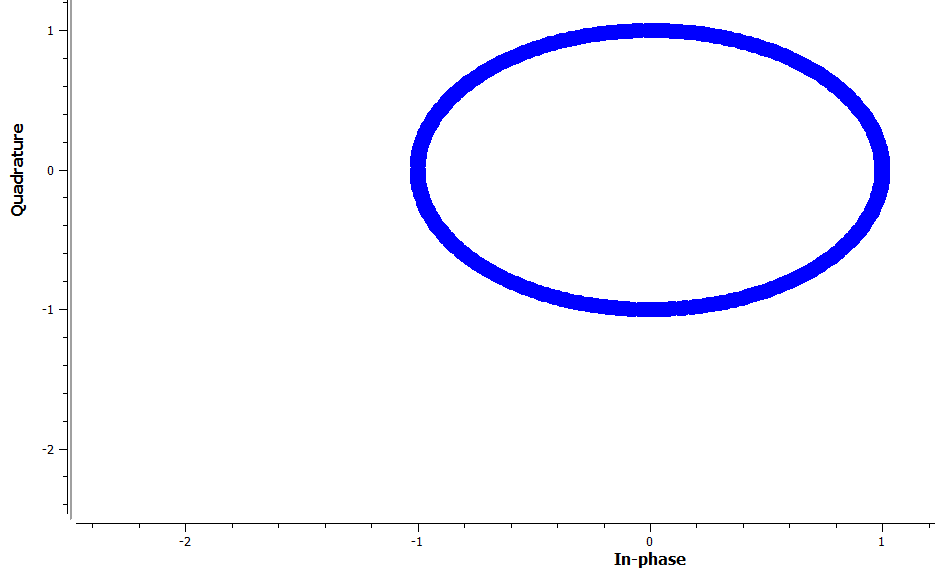
\includegraphics[width=0.6\columnwidth]{figs/FSK_constelation.png}
    \caption{FSK Constellation}
    \label{fig:figFSKconstellation}
\end{figure}

FSK modulation therefore maintains constant amplitude but encodes information 
through discrete frequency changes, which makes it less sensitive to amplitude 
noise but more dependent on accurate frequency separation.


% --- Transición desde la sección anterior (FSK) ---
After analyzing the OOK, BPSK, and FSK modulations, it is necessary to understand how 
the RF and complex envelope versions of the signals are generated inside GNU Radio. 
This process is carried out by two essential components: the \texttt{e\_RF\_VCO\_ff} 
and \texttt{e\_EC\_VCO\_fc} blocks, which are described below.

% --- Nueva sección completa que reemplaza "VCO Module Analysis" ---
\section{Analysis of the e\_RF\_VCO\_ff and e\_EC\_VCO\_fc blocks}

This section presents the internal analysis and understanding of the 
\texttt{e\_RF\_VCO\_ff} and \texttt{e\_EC\_VCO\_fc} blocks used in GNU Radio. 
Each block was opened using the ``Open in Editor'' option to review its Python 
implementation and internal help message. The following figures show the modified 
help code and a short explanation of their operation.

\subsection{e\_RF\_VCO\_ff Block}

This block is an RF Voltage-Controlled Oscillator (VCO) that generates a sinusoidal 
signal in the radio-frequency domain. The upper input controls the amplitude of the 
output, while the lower input controls the instantaneous phase or frequency. 
The output is a real-valued modulated waveform that represents the transmitted RF signal.
\begin{figure}[H]
    \centering
        \centering
        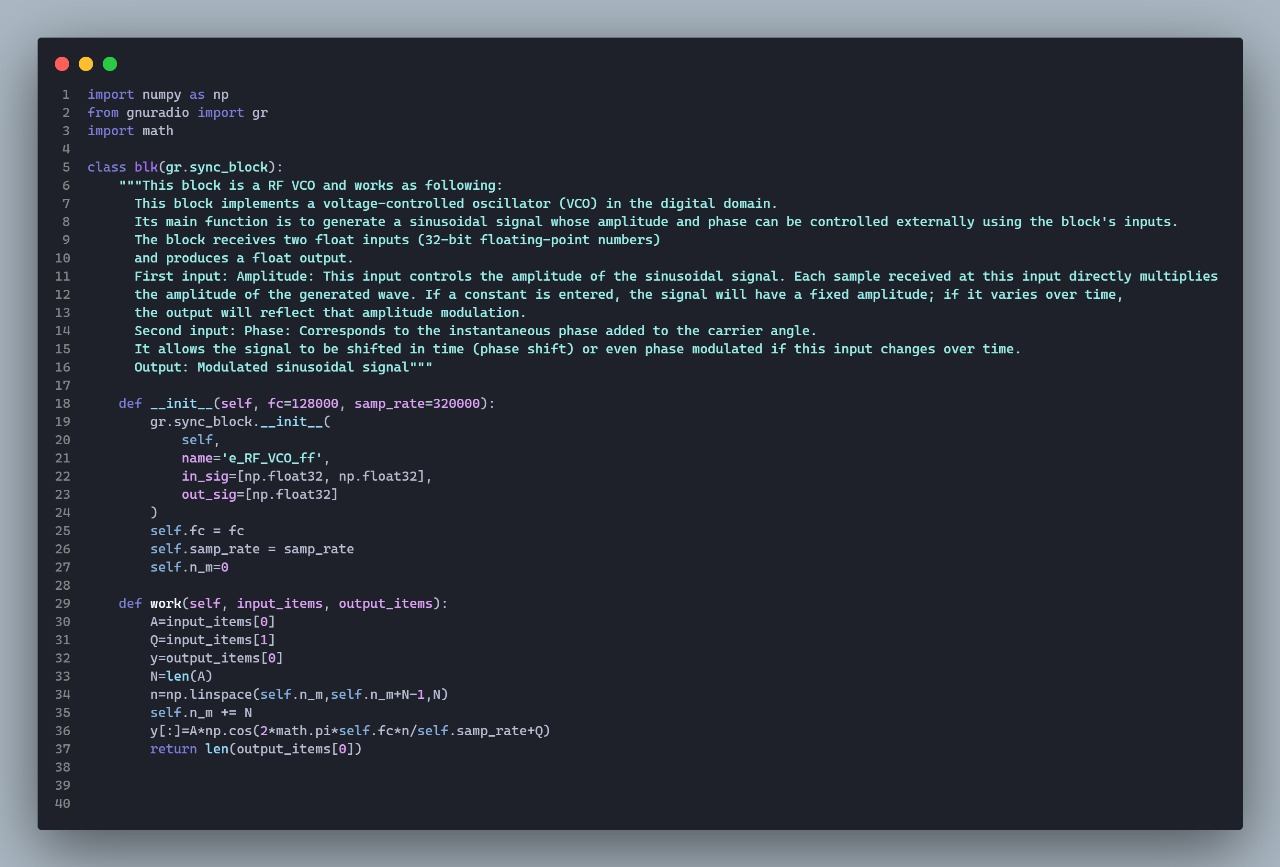
\includegraphics[width=0.6\columnwidth]{figs/codRF.jpg}
    \caption{e\_RF\_VCO\_ff} block opened in the GNU Radio editor. }
    \label{fig:codrf}
\end{figure}


\subsection{e\_EC\_VCO\_fc Block}

This block is a Complex Envelope Voltage-Controlled Oscillator (EC-VCO) that generates 
a baseband complex signal composed of in-phase (I) and quadrature (Q) components. 
The first input controls the amplitude, and the second input defines the phase of 
the complex output. The resulting signal simplifies the analysis of amplitude and 
phase variations in the complex plane.


\begin{figure}[H]
    \centering
        \centering
        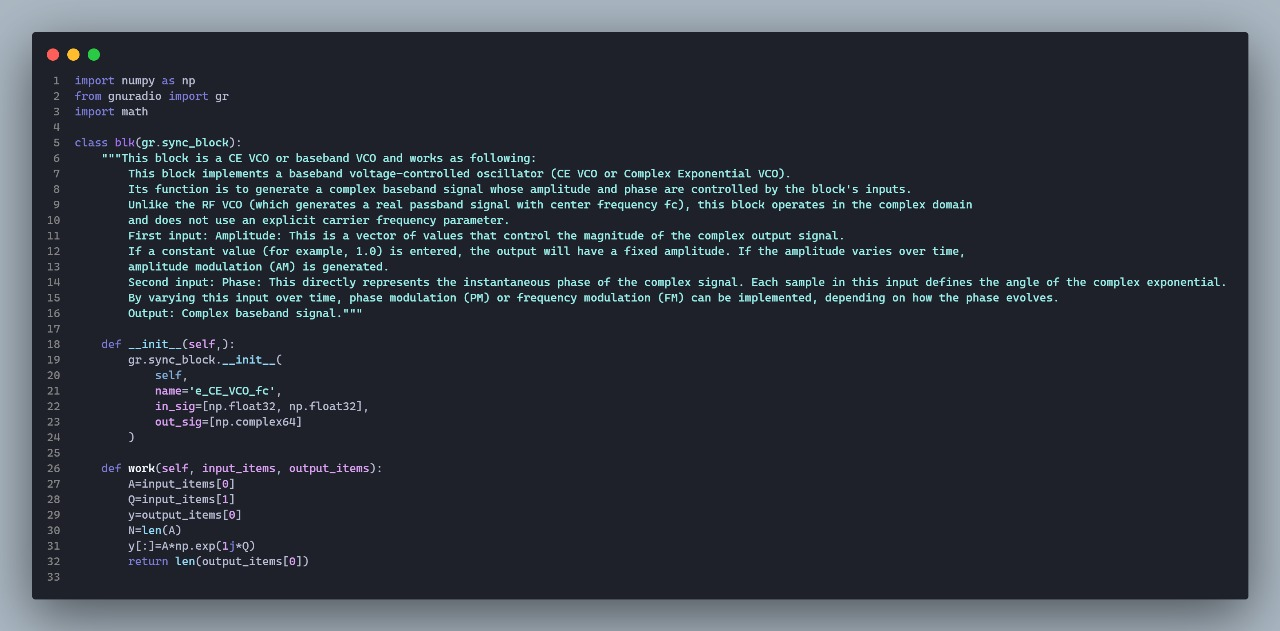
\includegraphics[width=0.6\columnwidth]{figs/codCE.jpg}
    \caption{e\_EC\_VCO\_fc} block opened in the GNU Radio editor. }
    \label{fig:codrf}
\end{figure}

\subsection{Comparison and Conclusion}

Both VCO blocks perform similar operations but in different domains. 
The \texttt{e\_RF\_VCO\_ff} produces a real RF signal that includes the carrier, 
while the \texttt{e\_EC\_VCO\_fc} generates its complex envelope representation. 
Together, they demonstrate the conversion between radio-frequency and complex envelope 
signals within the same modulation process.


\subsection{Control questions}
\begin{enumerate}
    \item This value was related to the sampling frequency; specifically, when using the plotting tool, the behavior of the signal with high frequency is shown in figure \ref{fig:figB}.

    \begin{figure}[H]
    \centering
        \centering
        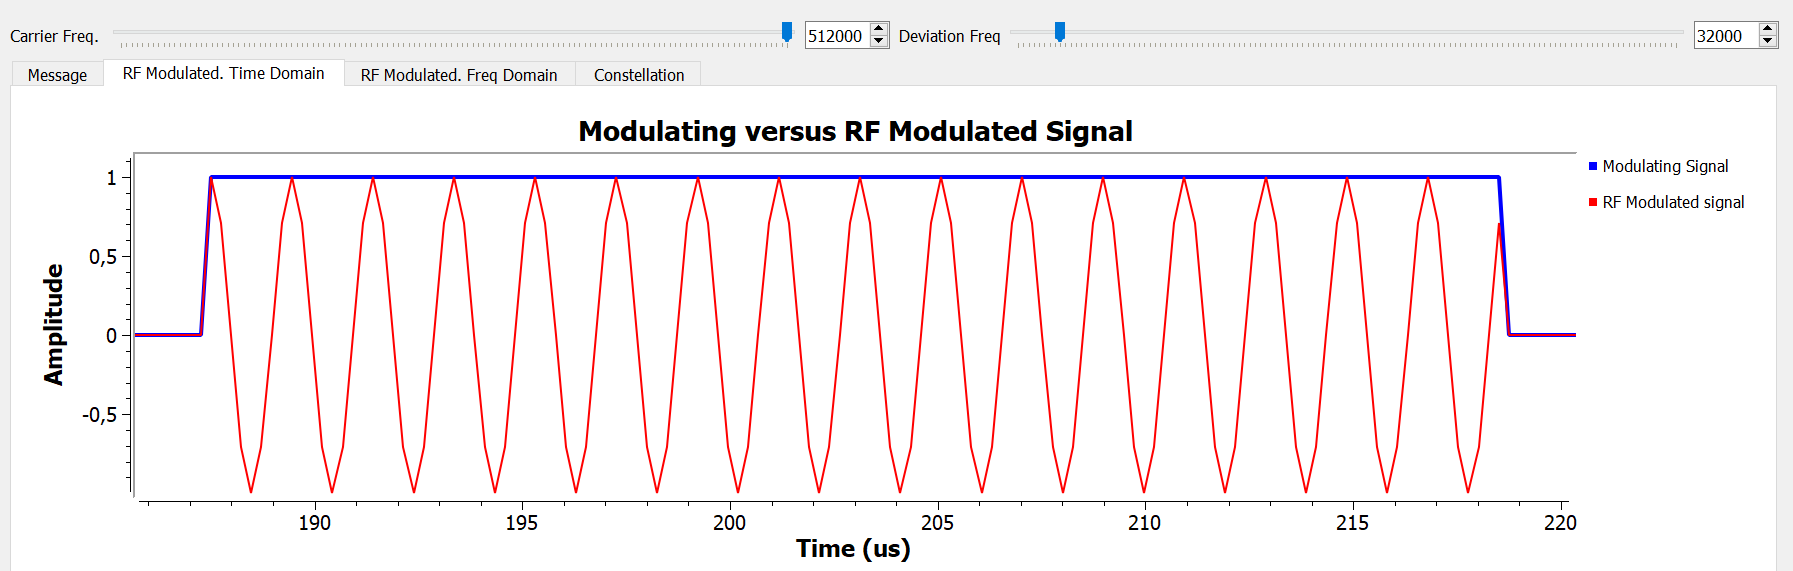
\includegraphics[width=0.6\columnwidth]{figs/VHF.png}
    \caption{Distortion due to the frequency approaching to the sample frequency}
    \label{fig:figB}
\end{figure}
    
    the message signal lost resolution or began to "distort".
    Thus, the SPS value would be determined by the frequency at which the message was intended to be transmitted via the carrier.\\
    
    For example, if a value of SPS = 128 was defined, the sampling frequency corresponded to 4.096MHz, limiting the bandwidth to which it could be transmitted maximally, also, being at this value was not very useful due to the resolution at that frequency. This led to transmitting the signal to approximately 1MHz to send information with sufficient resolution.

    \item When the \textit{Multiply Constant} block was removed from the flowchart, what happened is that the behavior of the BPSK modulation, the phase shift in the sinusoidal signal, was maintained, but the amplitude of the signal was halved. This would be a problem depending on the receiving system, as it may not have enough energy or amplitude to be well detected.

    \item The formula in the "Multiply Const" block corresponds to the bandwidth needed for FSK modulation, so the formula in the code: $2*math.pi*fd/Rb*sps$ finds this necessary bandwidth, the parameters $2*math.pi*fd$ corresponds to the offset frequency between the two carrier frequencies in FSK, $Rb$ represents the bit rate, in other words the rate at which the bits are sent, and $Sps$ corresponds to the samples per second.

    \item The constant source block in modulations implied a significant distinction, resulting in a different assigned value. For OOK modulation, this value referred to the system's phase. In this case, since OOK did not require such strict synchronization, the phase could be set at 0°. However, in the case of FSK, this value corresponded to the system's amplitude, as the phase was affected by other parameters. In FSK, the phase corresponded to a value that was integrated to obtain frequency modulation, meaning this value could not remain constant. This variability even implied that phase deviations impacted the signal, as they entered the integral that formed the block diagram represented in Figure \ref{fig:figA}.

    Although it was true that BPSK should have a constant source, in reality, this value should have been the phase, since if one used this value as the amplitude and the multiply constant as the phase, the result of BPSK ended up being incorrect. This was mainly due to the fact that the system, when we varied its phase, did not have a separation of 180° but only up to 90° or -90° according to the flowchart.
    something that did not occur in the case of using this block as the phase.

    \item OOK modulation is a variation of ASK modulation, a type of amplitude modulation, which is why the random source samples entered through the first input of both blocks, since this corresponds to the amplitude. Unlike FSK and BPSK, which are frequency and phase modulations, so the argument of the complex envelope concerning the phase changed, but the magnitudes remained constant.

    \item Implementing the mentioned change would not be correct because the result would be an oversampled signal, in which no parameters could be identified, by changing the "Interpolating FIR Filter block to be immediately before the VCO", what would be done is that first the "Multiply constant" block is multiplied to the signal and from there to the interpolation, which would cause the signal to be multiplied by a factor of the "Multiply constant" block.

    \item The answer was no, as the interpolation filter had the role of converting the bipolar digital signal starting from a random source into deterministic. This was important because the various changes in the signal due to its randomness would be affected by the summing block (representing the integral) and the proportionality constant, which in this case corresponded to the sensitivity coefficient of the modulator.
    
    When all of this was applied before and to a random signal, the effect was undesirable, with these phase changes in the signal because the transition between data would be completely random.

    \end{enumerate}

    \begin{enumerate}[label=\Alph*]

    \item The original code was slightly modified, changing the source input variable, no longer understood as the amplitude argument but as a constant multiplying the carrier frequency.
     Code: y[:]=1\*np.cos(\textbf{A}*2*math.pi*self.fc*n/self.samp\_rate+Q)

     The result was FSK modulation.
     
    \item In the code a maximum carrier value is set as $samp\_rate/8$ to avoid aliasing, but in the case where you want to know the maximum frequency at which the carrier can go it depends on two parameters, corresponding to $samp\_rate$ and the frequency deviation dev, so  $Freqmax = \frac{samp\_rate}{2} - dev$.
    
    \item Frequency deviation was a parameter of great importance for the application of FSK in the laboratory; it determined the frequency based on each logic according to a truth table. When a logical value of "1" was obtained, a frequency of $fc+fd$ was achieved, and when a "0" was obtained, a frequency of $fc-fd$ was achieved. At that moment, as observed in Figure X, the following could be concluded:

    \begin{figure}[H]
        \centering
            \centering
            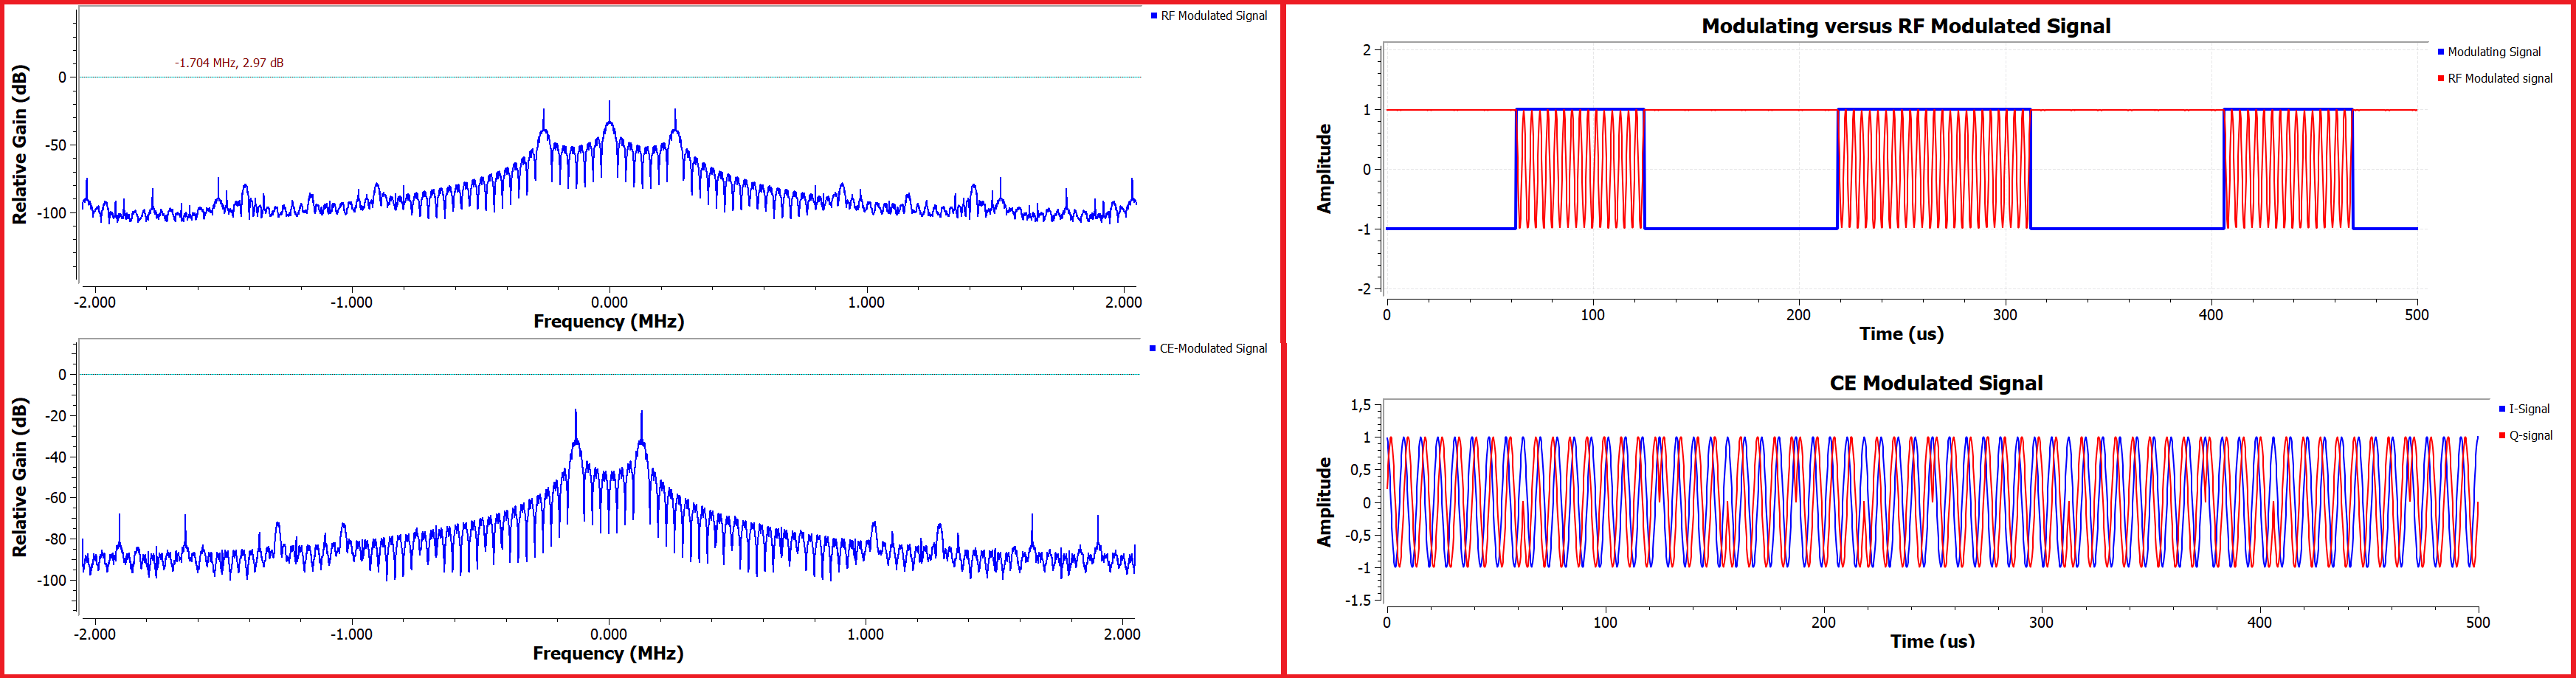
\includegraphics[width=0.7\columnwidth]{figs/Fd.png}
        \caption{Distortion due to the Frequency deviation approaching Rb*4}
        \label{fig:figB}
    \end{figure}

    Due to the initially corresponding separation between lobes of 32 kHz, if this frequency was increased to 128 kHz, a frequency of 0 Hz was achieved due to the logical "0". Beyond that, although it seemed that the behavior was restored, in reality, aliasing behavior was being obtained, which could be detrimental when demodulating the signal. This then left the frequency deviation limit in function to the carrier frequency. Additionally, if the sampling frequency were lower, there would also be the possibility that aliasing would be generated by the logical "1" component, but it would be defined in terms of this.

    \item In order to generate the BPSK modulation, two important parameters were taken into account, the SPS and the carrier frequency. Because the SPS was defined small and the desired frequency response was not obtained due to the very low frequencies that were allowed by fulfilling the Nyquist criterion. However, even if the number of SPS was increased, if the carrier frequency was small, the response was not obtained. It is important to say that increasing the SPS allowed to have a wider range of frequencies, increasing the upper and lower limits.

    A good approximation taken was that the number of samples per second should be such that the source signal is as close to a window as possible with an almost instantaneous rise time.

    \begin{figure}[H]
    \centering
        \centering
        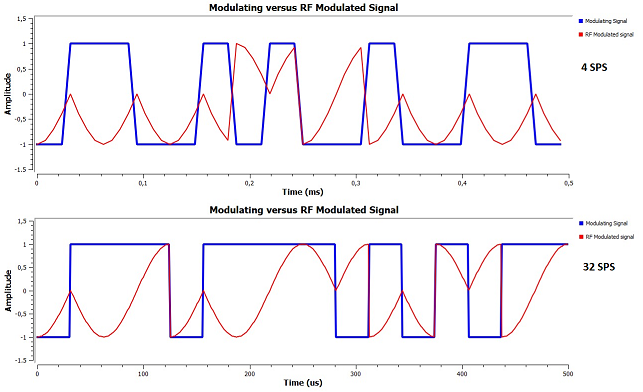
\includegraphics[width=0.6\columnwidth]{figs/PT_2_D_time.png}
    \caption{Comparison of BPSK modulation. 4 SPS vs. 32 SPS.}
    \label{pt_2_d}
    \end{figure}

    \begin{figure}[H]
    \centering
        \centering
        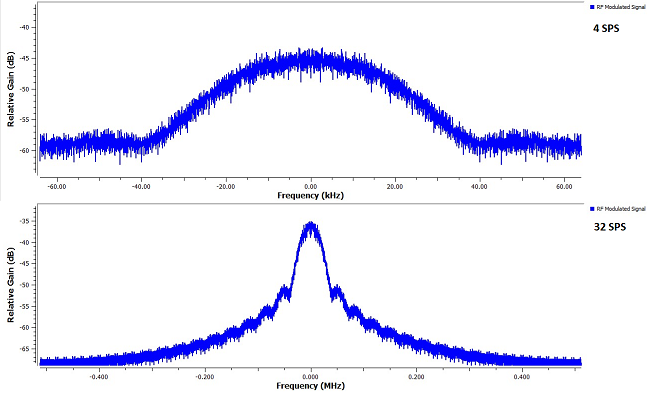
\includegraphics[width=0.6\columnwidth]{figs/PT_2_D_FREQ.png}
    \caption{Comparison of BPSK modulation frequency response at fc 8kHz. 4 SPS vs. 32 SPS.}
    \label{pt_2_d_freq}
    \end{figure}
    
\end{enumerate}

\section{Summary}

\begin{enumerate}
 \item The OOK modulation enabled the transmission of information through toggling the carrier on and off, thereby reducing power consumption. However, noise in the off state could prove detrimental. Depending solely on amplitude simplified demodulation, unaffected by frequency deviation. Compared to FSK and to some extent BPSK, it didn't require phase synchronization. Its constellation structure displayed phase and quadrature values coherent with the phasor position, easing analysis.

 \item In comparison to OOK, BPSK demonstrated that using two frequencies could be another way to transmit a message. However, due to its two oscillation states at 180° apart, it resulted in higher power consumption. Nevertheless, a benefit was the reduced noise observed. Like OOK, BPSK allowed for the identification of phase and quadrature through the use of two values, enabling their separation of 180° to be easily discerned on the constellation diagram.

 \item In comparison to BPSK and OOK, FSK exhibited distinct behavior, with its quality determined by frequency deviation. Unlike other modulations, where deviation and carrier frequency dictated code transmission, FSK's quality depended on frequency deviation, making phase synchronization a primary concern. Its identification of RF showed a deviation-dependent pattern, risking aliasing with excessive deviation. In its constellation diagram, FSK displayed a circumference due to minute changes, reflecting alternating phase cycles caused by significant frequency shifts unlike BPSK, which maintained a consistent frequency with a 180° phase offset.

 \item VCO blocks played a crucial role in determining the RF and EC signals, as they were responsible for setting up the carrier and breaking down the message components for modulation.
 
\end{enumerate}

% NO MODIFIQUE NI ELIMINE ESTA PARTE PARA QUE  APAREZCAN LAS REFERENCIAS
\bibliographystyle{IEEEtran}
\bibliography{bibliografia.bib}\nocite{*}

\end{multicols}
\end{document}